\documentclass{beamer}


\usepackage{kotex}
\usepackage{hyperref}
\usepackage{multirow}
\usepackage{graphicx}
\usepackage{amssymb,amsfonts,amsmath}
\usepackage[ps]{hfontsel} 
 \usepackage{setspace}
%\onehalfspacing


%\usetheme{Madrid} % Beamer theme v 3.0
  \setbeamertemplate{background canvas}[vertical shading][bottom=red!10,top=blue!10]
\usetheme{Warsaw}
 \usefonttheme[onlysmall]{structurebold}
%\usecolortheme{lily} % Beamer color theme
\setbeamercovered{dynamic}

\begin{document}

\author{조남운\\\url{mailto:namun.cho@gmail.com}}
\title{표와 그림}
\date{2008.2.19}

\begin{frame}
\maketitle
\end{frame}
%\setcounter{chapter}{3}
%\chapter{표와 그림}\label{ch:fig}

%\ref{ch:fig}장에서는 표와 그림을 다루는 방법에 대해 알아본다. 우선 간단한 그림을 하나 넣어보면서 \TeX에서 그림을 넣는 법\footnote{좀 더 정확하게는 떠다니는 개체(Floating Object)를 넣는 법이라고 해야 한다. \TeX에서는 모든 객체가 일종의 상자(Box)로 취급된다고 한다. 가장 작은 상자는 바로 글자이다. 표나 그림은 커다란 상자라고 보면 되겠다. 이 커다란 상자들을 통칭하여 떠다니는 개체라고 하며, 이것의 배치법은 일정한 규칙에 따른다. }에 대해서 알아보도록 하자. 


\section{그림 넣기}
\subsection{예제 1 : 간단한 그림 넣기}
%일단, \url{http://econ.korea.ac.kr/~hokyoung/valueTheory/bbs/data/renewal_bbs/abcd.jpg}에서 사진을 다운받고, \TeX 연습용으로 쓰고 있는 폴더에 넣어두자. 그리고 아래와 같이 입력해본다. 
\begin{frame}
\begin{block}{가장 간단한 그림 넣기 }
\begin{enumerate}[1{단계}.]
\item <1-> \url{http://econ.korea.ac.kr/~hokyoung/valueTheory/bbs/data/renewal_bbs/abcd.jpg}에서 사진을 다운받는다.
\item <2->\TeX 연습용으로 쓰고 있는 폴더에 넣어둔다. 
\item <3->다음과 같이 입력해본다. 
\end{enumerate}
\end{block}
\end{frame}

\begin{frame}[fragile]
\begin{block}{첫번째 입력 예제}
\begin{verbatim}
\begin{figure}[htbp]    %그림의 시작을 알림과 동시에 자리배치에 대한 원칙이 [htbp]로 전달되었다. 
  \begin{center}	     %그림의 가로위치를 가운데로 정렬함.  
    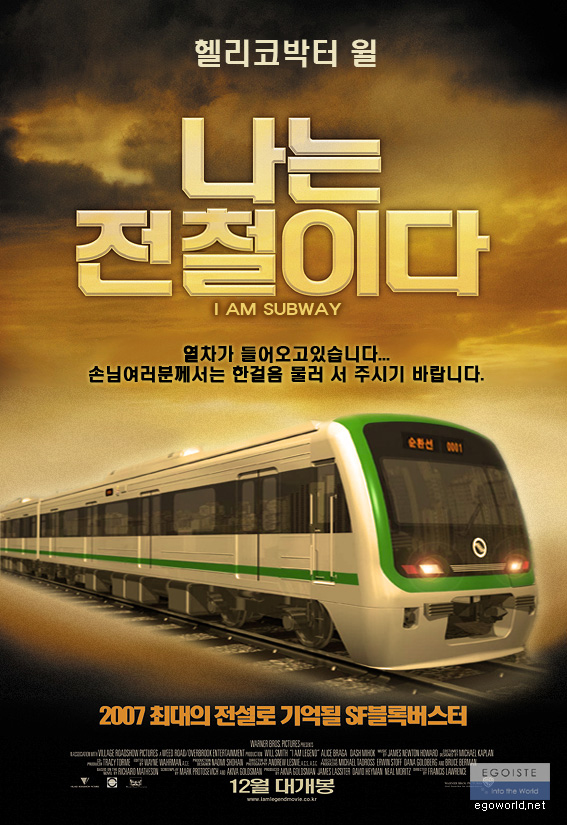
\includegraphics[width=0.2\textwidth]{abcd}    %그림 파일의 위치와 배치크기옵션. 여기에서는 종이의 가로폭의 20퍼센트를 지정함. 
  \caption{나는 전철이다 ㅋㅋ}  %그림 설명글(캡션). 별도 지정이 없으면 아래쪽에 표시됨.
  \label{fig:iamsubway} %참조용 레이블. 그림 #으로 부를 때 그 #을 \ref{fig:iamsubway}로 한다. label은 겹치지만 않으면 된다. 즉, \label{aaa} 같은 식으로 써도 무방하다. 
  \end{center}
\end{figure}
\end{verbatim}
\normalsize
\end{block}
\end{frame}

\begin{frame}
\begin{block}{첫번째 입력 예제의 결과}
\begin{figure}[htbp]
  \begin{center}
    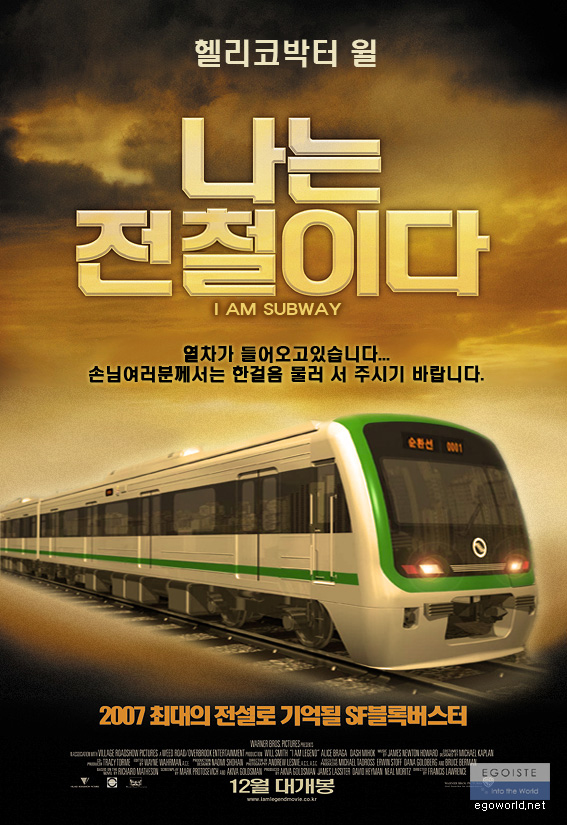
\includegraphics[width=0.2\textwidth]{abcd}
  \caption{나는 전철이다 ㅋㅋ}
  \label{fig:iamsubway}
  \end{center}
\end{figure}
\end{block}
\end{frame}

\begin{frame}[fragile]
%아마도 그림은 원하는 위치에 오지 않았을 것이다. \TeX는 기본적으로 이러한 표나 그림의 배치 등도 자동으로 위치를 잡는 알고리즘에 따라 자동 배치를 한다. 물론 수동으로 정확하게 자신이 의도한 자리에 의도한 배치를 하게 할 수는 있지만, 그것은 직접 기술 문서를 참조하면 알 수 있다. 


%위의 실습용 예문에 주를 달아두긴 했지만, 다시 설명해보도록 하자. 
%\begin{table}[H!]
%\caption{그림 구문}
%\begin{center}
%\begin{tabular}{c|c}
%\toprule
%\text{\begin{verbatim}\begin{figure}[htbp]\end{verbatim}}& \text{   그림의 시작을 알림과 동시에 자리배치에 대한 원칙이 [htbp]로 전달되었다.} \\
%\text{\begin{verbatim}  \begin{center}	    \end{verbatim}} &\text{그림의 가로위치를 가운데로 정렬함. } \\
%\text{\begin{verbatim}    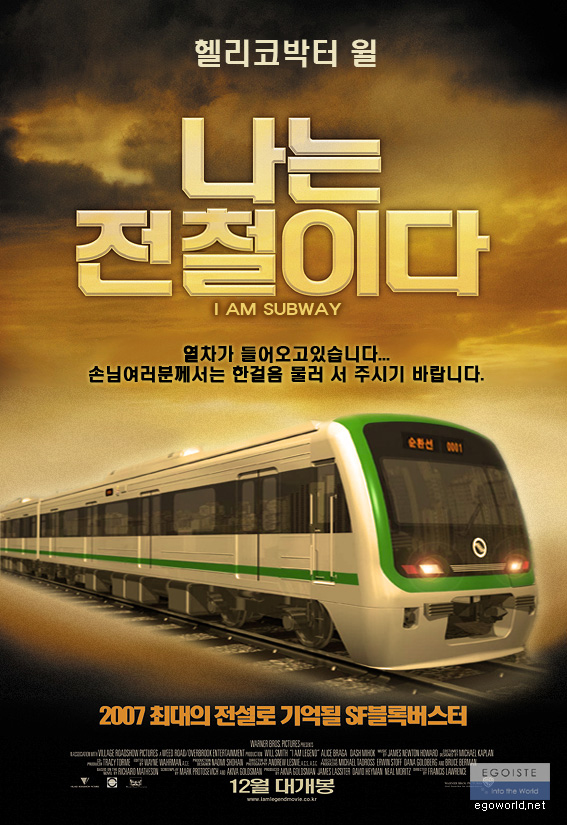
\includegraphics[width=0.2\textwidth]{abcd} \end{verbatim}}   &\text{그림 파일의 위치와 배치크기옵션. 여기에서는 종이의 가로폭의 20퍼센트를 지정함. }\\
%\text{\begin{verbatim}  \caption{나는 전철이다 ㅋㅋ} \end{verbatim}} &\text{그림 설명글(캡션). 별도 지정이 없으면 아래쪽에 표시됨.}\\
%\text{\begin{verbatim}  \label{fig:iamsubway} \end{verbatim}}&\text{참조용 레이블. 그림 \#으로 부를 때 그 \#을 \begin{verbatim}\ref{fig:iamsubway}\end{verbatim}로 한다. label은 겹치지만 않으면 된다. }\\
%\text{\begin{verbatim}  \end{center}\end{verbatim}}\\
%\text{\begin{verbatim}\end{figure}\end{verbatim}}\\

%\bottomrule
%\end{tabular}
%\end{center}
%\label{default}
%\end{table}%

%위 예제에서 알 수 있듯 가장 중요한 부분은 {\verb|\begin{figure}[htbp]|}이다. 이 htbp는 h, t, b, p라는 옵션을 사용한다는 것을 의미하는데, 각각 h는 바로 이 자리(here), t는 문서의 최상단(top), b는 문서의 최하단(bottom), p는 별도의 그림만 모아놓은 장(page)를 의미한다. \TeX에는 미리 정의된, 떠다니는 개체의 크기에 따른 배치 조건이 설정되어 있으며, 이를 어기면 우선순위에 따라 다음 조건을 탐색하게 된다. 모든 탐색조건을 충족하지 못한다면, 그 경우 p 옵션이 발동되어 떠다니는 개체만을 모은 페이지로 가게 된다. 만일 이 알고리즘 조건을 무시하고 싶다면 `!'를 붙이면 된다. 특히, 절대 조건과 상관없이 이자리로 가게 하고 싶을 경우 [h!] 옵션을 사용한다. 아무 옵션도 붙이지 않으면 tbp로 설정된다. 
\begin{block}{위치 지정자 htbp}<1->
\begin{itemize}
\item <1->\verb|\begin{figure}[htbp]|
\item <2->h : 바로 이 자리
\item <2->t : 페이지 상단, b : 하단, p : 별도 페이지
\item <3->위 옵션 중 적당한 것을 \TeX에서 지정해줌
\item <4->만일 자동 지정을 무시하고 강제로 넣고 싶은 경우, ``!''를 앞에 붙임. ex) [!h]
\end{itemize}

\end{block}
%들어갈 그림파일의 위치는 \verb|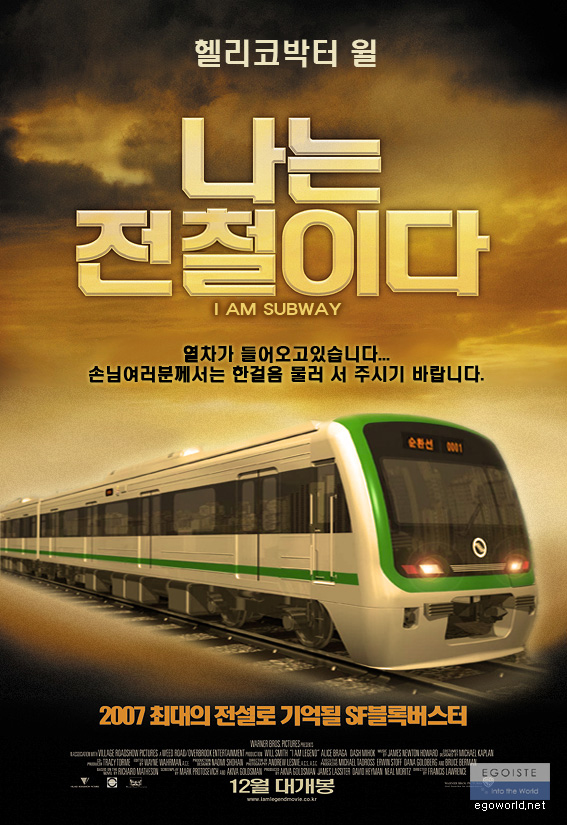
\includegraphics[width=0.2\textwidth]{abcd}|에 명시되어 있다. 파일 이름의 확장자는 써도 되지만, 명시하지 않아도 무방하다. \TeX는 파일명 뒤에 자신이 지원하는 그림 파일 확장자를 붙여가며 탐색을 하기 때문이다. 다만, EPS확장자는 지원하지 않으므로 미리 pdf나 jpg 등으로 변환시켜두어야 한다. 대괄호 안의 \verb|width=0.2\textwidth|는 폭을 문서 가로폭의 20\%로 하겠음을 명시하는 것이다. 당연히 0.2를 가령 0.5로 만들면 폭의 50\%만큼의 그림이 되는 것이다. 
\begin{block}{그림파일 넣는 부분}<5->
\verb|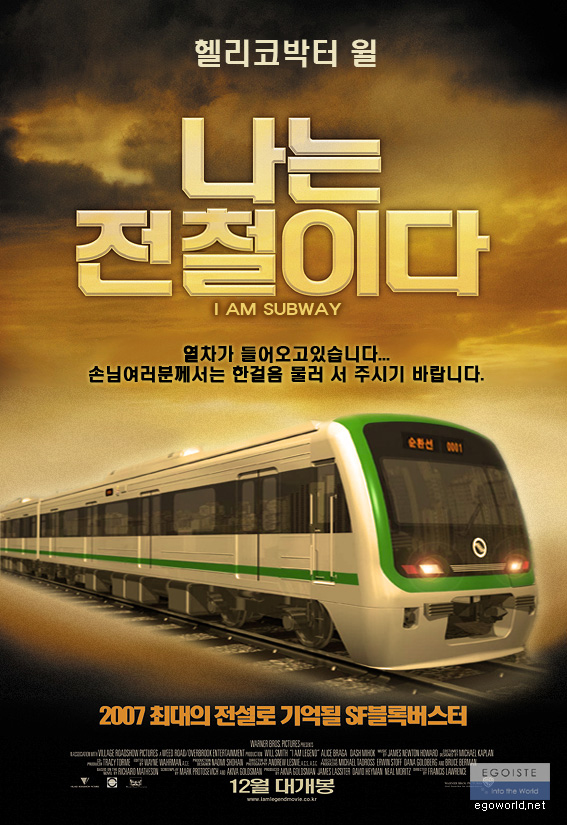
\includegraphics[width=0.2\textwidth]{abcd}|
\end{block}
\end{frame}



\begin{frame}[fragile]
\begin{block}{그림 옵션 변경}
\begin{verbatim}
\begin{figure}[h!]
  \begin{center}
    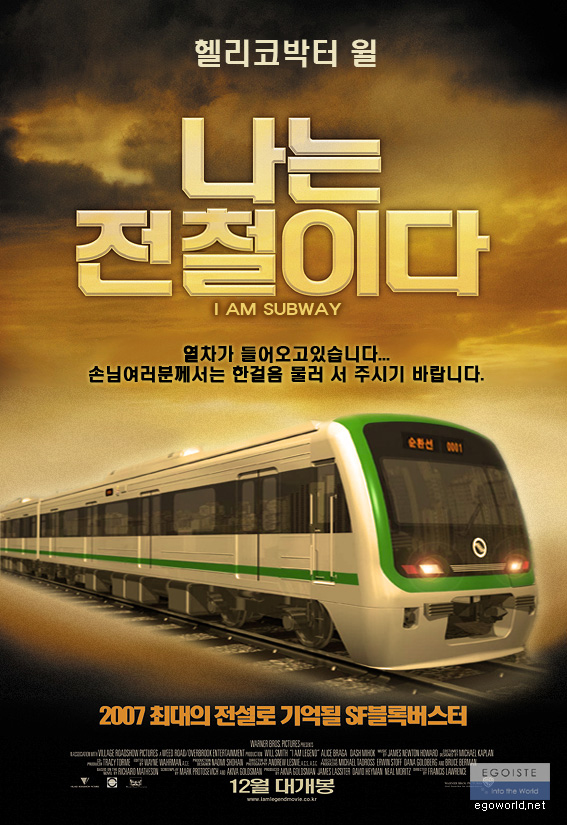
\includegraphics[angle=90, width=0.9\textwidth]{abcd}
  \caption{상대크기를 폭의 90\%로 확대하면서 반시계방향으로 90도 꺾음}
  \label{fig:iamsubway}
  \end{center}
\end{figure}
\end{verbatim}
\end{block}
\end{frame}

\begin{figure}[h!]
  \begin{center}
    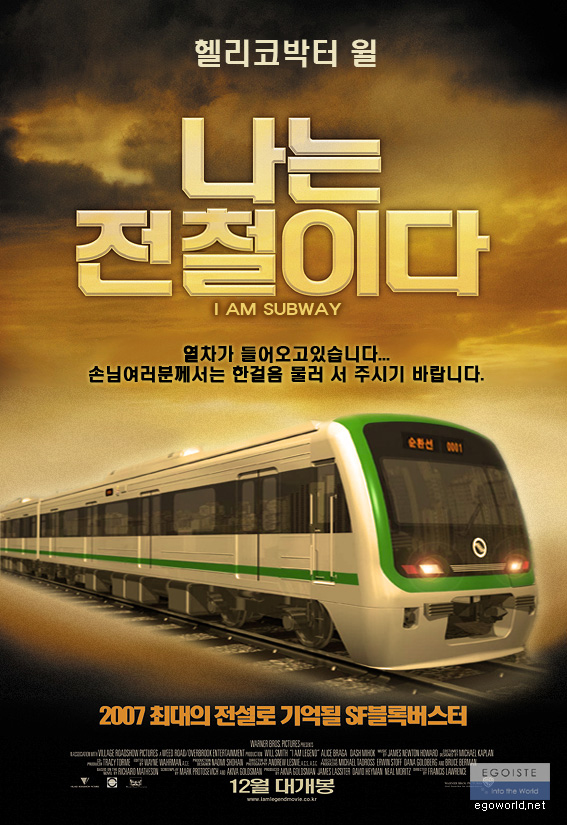
\includegraphics[angle=90, width=0.9\textwidth]{abcd}
  \caption{상대크기를 폭의 90\%로 확대하면서 반시계방향으로 90도 꺾음}
  \label{fig:iamsubway}
  \end{center}
\end{figure}

\section{표 만들기}
%표는 tabular환경을 사용한다. 

\subsection{간단한 표의 예}

\begin{frame}[fragile]
\begin{block}{간단한 표의 예}
\begin{columns}
\begin{column}{0.5\textwidth}
  \begin{verbatim}
  \begin{center}
  \begin{tabular}{|c||c|c|}
  \hline  
  & 자백 & 부인 \\
  \hline \hline
  자백 & 5,5 & 1,100 \\
  \hline 
  부인 & 100,1 & 0,0 \\
  \hline 
  \end{tabular}
  \end{center}
\end{verbatim}
\end{column}

\begin{column}{0.5\textwidth}
\begin{center}
\begin{tabular}{|c||c|c|}
\hline  
& 자백 & 부인 \\
\hline \hline
자백 & 5,5 & 1,100 \\
\hline 
부인 & 100,1 & 0,0 \\
\hline 
\end{tabular}
\end{center}
\end{column}


\end{columns}

\end{block}
\end{frame}

%위 문장을 실행시키면 아래와 같은 결과를 얻을 것이다. 이는 그림과 유사하지만, 위치 지정자(htbp)나  가운데 정렬방식 등을 설정하지 않았으므로 거대한 한 글자와 같이 취급되고 있다. 그래서 부자연스럽게 같은 줄에 위치하고 있다. 이것을 피하기 위해서는 \verb|\begin{center}\end{center}|같은 정렬 명령을 쓴다. 이는 수식의 \verb|$수식$|과 equation환경(\verb!\begin{equation*}\end{equation*}!)을 쓰는 수식의 차이와 유사하다고 생각하면 된다. 


\begin{frame}

\begin{block}{가로선과 세로선의 관계}
\begin{columns}
\begin{column}{0.5\textwidth}
\begin{figure}[!h]
\begin{center}
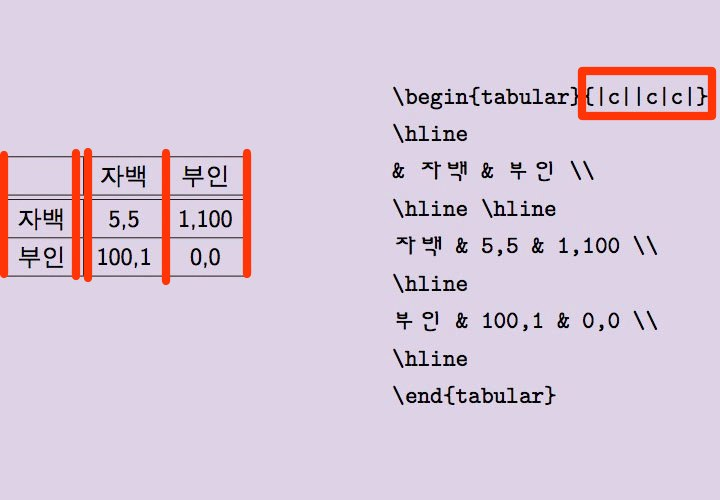
\includegraphics[width=0.9\textwidth]{table001}
%\caption{default}
%\label{default}
\end{center}
\end{figure}

\end{column}
\begin{column}{0.5\textwidth}
\begin{figure}[!h]
\begin{center}
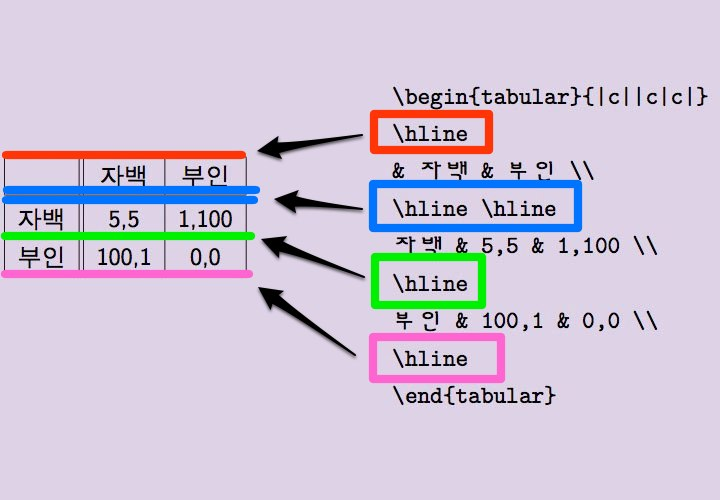
\includegraphics[width=0.9\textwidth]{table002}
%\caption{default}
%\label{default}
\end{center}
\end{figure}

\end{column}
\end{columns}
\end{block}
\end{frame}

%표의 내용을 채우고 있는 부분은 수식의 행렬과 매우 유사한데, 행 구분은 \verb|\\|으로, 열 구분은 \&로 하고 있다. 주의할 점은, 아무것도 없는 부분(여기에서는 1행 1열이 그러하다)이 비었다는 것을 표현하기 위해 \& 자백 \& 부인 \verb|\\| 같은 식으로 표현한다는 점이다. \verb!\begin{tabular}{|c||c|c|}!의 의미는 가운데 정렬(center)을 하는 3열짜리 표라는 것이며, 세로줄을 모두 긋되, 1열과 2열 사이의 세로줄은 두줄짜리를 쓰겠다는 것을 의미한다. 즉, 처음 표를 시작할 때 열에 대한 정보와 함께 세로선에 대한 기본 정보를 제공하는 것이라고 생각하면 된다. 가로선은 \verb!\hline! 명령을 쓴다. 

%위에서 쓴 c대신 쓸 수 있는 것은 l, r, p 등이 있다. l은 왼쪽정렬(left), r은 오른쪽 정렬(right), p는 줄바꿈이 가능하게 한다(paragraph). 뒤에 중괄호를 붙여 크기를 강제로 지정할 수 있다. 지정하지 않는 경우 \LaTeX이 자동으로 폭을 결정해주게 된다. %paragraph와 가운데 정렬 등의 조합법 찾아 넣을 것.  

\subsection{조금 더 복잡한 표}
%좀 더 복잡한 표를 만들어 보자. 

\subsubsection{열병합 표}
%열 병합은 multicolumn 명령을 사용한다. 

\begin{frame}[fragile]
\begin{block}{열병합 표}
\small
\begin{verbatim}
\begin{table}[!h]
\begin{center}
\begin{tabular}{|c|c|c|}
\hline
\multicolumn{3}{|c|}{종   류}\\
\cline{1-3}
C1&C2&C3\\
\hline
2.1&2.2&2.3\\
\cline{2-3}
3.1&3.2&3.3\\
\hline
\end{tabular}
\end{center}
\end{table}
\end{verbatim}
\end{block}
\end{frame}

\begin{frame}
\begin{block}{결과}
\begin{table}[!h]
\begin{center}
\begin{tabular}{|c|c|c|}
\hline
\multicolumn{3}{|c|}{종   류}\\
\cline{1-3}
C1&C2&C3\\
\hline
2.1&2.2&2.3\\
\cline{2-3}
3.1&3.2&3.3\\
\hline
\end{tabular}
\end{center}
\end{table}
\end{block}
\end{frame}

\begin{frame}
\begin{block}{cline명령}
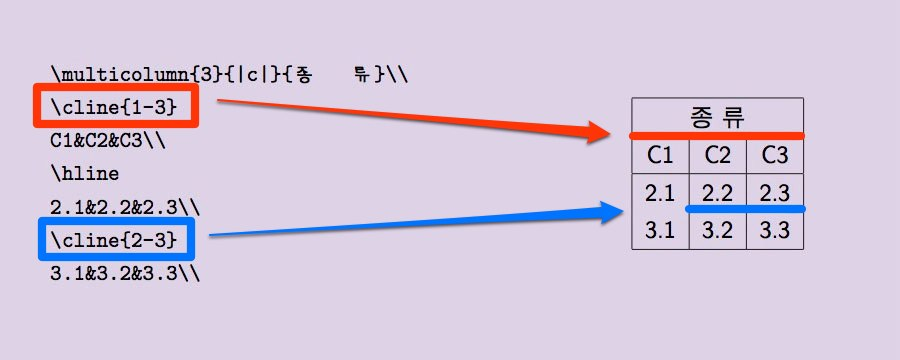
\includegraphics[width=0.9\textwidth]{table2-001}
\end{block}
\end{frame}

%위 표의 미완성된 줄은 일부러 그은 것이다. \verb!\cline{}! 명령어는 가로선의 시작부분과 끝부분을 지정한다. 즉, 위 예에서 세번째 셀의 중간에 걸친 밑선은 2번째 셀에서 시작하여 세번째 셀에서 끝나므로 \verb!\cline{2-3}!을 쓴 것이다. 



\subsubsection{행병합 표}
%이제 감을 잡았을 것이다. 행병합은 multirow 명령을 사용한다. 이때 multirow 명령을 사용한 cell은 빈 셀 취급을 하면 된다. 


\begin{frame}
\begin{block}{행병합 표}
\begin{table}[!h]
\begin{center}
\begin{tabular}{|l|l|l|l|}\hline
\multirow{3}{20mm}{Text in column1}&C2a&\multirow{4}{20mm}{Text in column3}&C4a\\
	&	C2b	&	&	C4b\\
	&	C2c	&	&	C4c\\
\cline{1-2}
C1d	&	C2d	&	&	C4d\\
\hline
\end{tabular}
\end{center}
\end{table}
\end{block}
\end{frame}


\begin{frame}[fragile]
\begin{block}{행병합 표 소스}
\begin{center}
\begin{verbatim}
\begin{table}[!h]
\begin{center}
\begin{tabular}{|l|l|l|l|}\hline
\multirow{3}{20mm}{Text in column1}&C2a&
\multirow{4}{20mm}{Text in column3}&C4a\\
	&	C2b	&	&	C4b\\
	&	C2c	&	&	C4c\\
\cline{1-2}
C1d	&	C2d	&	&	C4d\\
\hline
\end{tabular}
\end{center}
\end{table}
\end{verbatim}
\end{center}
\end{block}
\end{frame}
%\subsubsection{표 속에 표를 넣기}

%\subsubsection{표 속에 각주 넣기}

\begin{frame}

\begin{itemize}
\item[] 
\begin{center}
수고하셨습니다!!
\end{center}
\end{itemize}


\end{frame}

\end{document}


